\documentclass[reprint,english,notitlepage,aps,nobalancelastpage,nofootinbib]{revtex4-1}
\usepackage[utf8]{inputenc}
\usepackage[english]{babel}
\usepackage{physics,amssymb}
\usepackage{graphicx}
\usepackage{xcolor}
\usepackage{hyperref}
\usepackage{tikz}
\usepackage{listings}
\usepackage{subfigure}
\usepackage{amsmath,mathtools}
\usepackage{amsbsy}
\usepackage{enumitem}
\usepackage{bbold}

\graphicspath{{../plots/}}

\hypersetup{
    colorlinks,
    linkcolor={red!50!black},
    citecolor={blue!50!black},
    urlcolor={blue!80!black}}

\lstset{
	inputpath=,
	backgroundcolor=\color{white!88!black},
	basicstyle={\ttfamily\scriptsize},
	commentstyle=\color{magenta},
	language=Python,
	morekeywords={True,False},
	tabsize=4,
	stringstyle=\color{green!55!black},
	frame=single,
	keywordstyle=\color{blue},
	showstringspaces=false,
	columns=fullflexible,
	keepspaces=true}


\newcommand{\closed}[1]{\left(#1\right)}
\newcommand{\bracket}[1]{\left[#1\right]}

\newcommand{\kt}{\kappa_T}
\renewcommand{\cp}{c_P}
\newcommand{\cv}{c_V}
\renewcommand{\a}{\alpha}

\newcommand{\tmdv}[4]{\closed{\pdv{#1}{#2}}_{#3,#4}}
\newcommand{\jacobian}[2]{\pdv{(#1)}{(#2)}}
\renewcommand{\d}{\mathrm{d}}

\newcommand{\nx}{N_x}
\newcommand{\ny}{N_y}
\newcommand{\nz}{N_z}
\newcommand{\V}{\tilde{V}}
\renewcommand{\P}{\tilde{P}}

\newcommand{\np}{N_+}
\newcommand{\kb}{k_B}

\begin{document}
\begin{center}
\title{\Huge FYS4130 - Oblig 1}
\author{\large Vetle A. Vikenes}
\date{\today}
\noaffiliation


\maketitle
\end{center}
\onecolumngrid

All code used in this oblig can be found on my Github: \url{https://github.com/Vikenes/FYS4130}
\\
\section*{\large Task 1 - Black box numerical method}
We want to find the isothermal compressibility at constant $T$ and $N$,
\begin{align} \label{eq:kappa black box}
	\kt = -\frac{1}{V}\closed{\pdv{V}{P}}_{T,N},
\end{align}
with a black box numerical method which gives us values for $P$ and $N$ as function of intput parameters $T,\,V,$ and $\mu$ which we may vary. The derivatives we're able to compute with our numerical method is the partial derivative of either $P$ or $N$ with respect to one of the input parameters, when the other two are held constant. We must therefore rewrite equation \eqref{eq:kappa black box}, such that it only contains such derivatives. To begin, we use the chain rule on the reciprocal of the partial derivative in equation \eqref{eq:kappa black box}
\begin{align*}
	\tmdv{P}{V}{T}{N} &= \jacobian{P,T,N}{V,T,N}=\jacobian{P,T,N}{V,T,\mu}\cdot\jacobian{V,T,\mu}{V,T,N} \\
	&= \jacobian{P,N,T}{V,\mu,T}\cdot\jacobian{\mu,V,T}{N,V,T}=
	\jacobian{P,N,T}{V,\mu,T} \Big/ \tmdv{N}{\mu}{V}{T}.
\end{align*}
The last factor is a partial derivative we're able to compute, by computing the change in $N$ as we vary $\mu$ only. For the other factor, we expand the jacobian, using its definition 

\begin{align}
	\jacobian{P,N,T}{V,\mu,T} &= \tmdv{P}{V}{\mu}{T}\tmdv{N}{\mu}{V}{T}-\tmdv{P}{\mu}{V}{T}\tmdv{N}{V}{\mu}{T}. \label{eq:d PNT_d VmuT}
\end{align}
We see that the four partial derivatives in equation \eqref{eq:d PNT_d VmuT} are taken with respect to either $V$, with the other input parameters held constant, or $\mu$ with the other input parameters held constant. Measuring the change in $P$ and $N$ with these constraints is thus something our numerical method is capable of, and we have successfully reduced $\kt$ into multiple partial derivatives we're able to solve. The resulting expression for $\kt$ becomes  

\begin{align*}
	\kt &= -\frac{1}{V}\bracket{\jacobian{P,N,T}{V,\mu,T} \Big/ \tmdv{N}{\mu}{V}{T}}^{-1}=-\frac{1}{V} \tmdv{N}{\mu}{V}{T} \Big/
	\jacobian{P,N,T}{V,\mu,T} \\
	&= -\frac{1}{V} \tmdv{N}{\mu}{V}{T} \bracket{\tmdv{P}{V}{\mu}{T}\tmdv{N}{\mu}{V}{T}-\tmdv{P}{\mu}{V}{T}\tmdv{N}{V}{\mu}{T}}^{-1}.
\end{align*}

\clearpage
\section*{\large Task 2 - Partial derivative}
We want to rewrite the partial derivative 
\begin{align*}
	\tmdv{P}{U}{G}{N}.
\end{align*}
In this task we will need the standard set of second derivatives given in Swendsen, and we list them here for convenience
\begin{align}
	\a &= \frac{1}{V} \tmdv{V}{T}{P}{N} \label{eq:alpha} \\ 
	\kt &= -\frac{1}{V} \tmdv{V}{P}{T}{N} \label{eq:kappa} \\ 
	\cp &= \frac{T}{N} \tmdv{S}{T}{P}{N} \label{eq:cp} \\ 
\end{align}
We begin by applying the chain rule to the Jacobian, which enables us to get a partial derivative containing $U$ and $G$ in the denominator only. 

\begin{align} 
	\tmdv{P}{U}{G}{N} &= \jacobian{P,G,N}{U,G,N} = \jacobian{P,G,N}{P,T,N}\cdot\jacobian{P,T,N}{U,G,N}= \tmdv{G}{T}{P}{N} \jacobian{P,T,N}{U,G,N} \nonumber \\
	&= -S \Big/\jacobian{U,G,N}{P,T,N}, \label{eq:pdv first expansion}
\end{align}
where we used the differential form of the Gibbs free energy, $\mathrm{d}G=-S\mathrm{d}T+V\mathrm{d}P+\mu\mathrm{d}N$, to solve the first partial derivative of $G$ with respect to $T$ at constant $P$ and $N$. The second factor was written in terms of the reciprocal such that the thermodynamic potentials in the Jacobian appear in the nominator. 

We will now find an expression for $\pdv*{(U,G,N)}{(P,T,N)}$. To avoid partial derivatives containing $U$ and $G$ simultaneously, we expand the expression by using the definition of Jacobians. 

\begin{align}
	\jacobian{U,G,N}{P,T,N} &= \tmdv{U}{P}{T}{N} \tmdv{G}{T}{P}{N} - \tmdv{U}{T}{P}{N}\tmdv{G}{P}{T}{N} \nonumber \\ 
	&= -S\tmdv{U}{P}{T}{N} - V \tmdv{U}{T}{P}{N}, \label{eq:d UGN_d PTN}
\end{align}
where the last equation follow from the definition of $\d G$ and the partial derivatives of it. 

For the partial derivative of $U$ with respect to $T$ at constant $P$ and $N$, we consider the differential form of fundamental relation in the energy representation, which at constant $N$ becomes 

\begin{align}
	\d U &= T \d S - P \d V \nonumber \\ 
	\implies \tmdv{U}{T}{P}{N} &= T \tmdv{S}{T}{P}{N} - P \tmdv{V}{T}{P}{N} \nonumber \\ 
	&= N\cp - PV\a, \label{eq:dU_dT}
\end{align}
where we used equations \eqref{eq:cp} and \eqref{eq:alpha} for the two partial derivatives. 

For the partial derivative of $U$ with respect to $P$ with $T$ and $N$ held constant we apply the chain rule
\begin{align}
	\tmdv{U}{P}{T}{N} &= \jacobian{U,T,N}{P,T,N} = \jacobian{U,T,N}{V,T,N}\cdot \jacobian{V,T,N}{P,T,N} = \tmdv{U}{V}{T}{N} \tmdv{V}{P}{T}{N} \nonumber \\
	&= \tmdv{U}{V}{T}{N}(-V\kt). \label{eq:dU_dP}
\end{align}
Equation \eqref{eq:kappa} was used to rewrite the second partial derivative. For the other partial derivative, we once again use the previouslly mentioned expression for $\d U$ with $N$ held constant 
\begin{align} \label{eq:dU_dV}
	\tmdv{U}{V}{T}{N} &= T \tmdv{S}{V}{T}{N} - P.
\end{align}
To proceed with the final partial derivative we will first use a Maxwell relation. We notice that $S$ is differentiated with respect to $V$ at constant $T$ and $N$, so we can use the differential form of the Helmholtz free energy to derive the Maxwell relation. 
\begin{align*}
	\d F &= -S \d T -P \d V + \mu \d N \implies -\tmdv{F}{T}{V}{N} = S \\ 
	\tmdv{S}{V}{T}{N} &=-\bracket{\pdv{V}\tmdv{F}{T}{V}{N}}_{T,N} = -\bracket{\pdv{T}\tmdv{F}{V}{T}{N}}_{V,N} = \tmdv{P}{T}{V}{N}.
\end{align*} 
We rewrite the last partial derivative using the chain rule 
\begin{align}
	\tmdv{P}{T}{V}{N} &= \jacobian{P,V,N}{T,V,N} = \jacobian{P,V,N}{P,T,N}\cdot \jacobian{P,T,N}{T,V,N} = -\jacobian{V,P,N}{T,P,N}\cdot \jacobian{P,T,N}{V,T,N} \nonumber \\ 
	&= -\tmdv{V}{T}{P}{N} \Big/ \tmdv{V}{P}{T}{N} = -V\a \big/ (-V\kt) = \frac{\a}{\kt}, \label{eq:alpha_kappa}
\end{align} 
where in the last step equations \eqref{eq:alpha} and \eqref{eq:kappa} were used to rewrite the nominator and denominator, repsectively. Equation \eqref{eq:dU_dP} can now be solved, by inserting equation \eqref{eq:alpha_kappa} into equation \eqref{eq:dU_dV} 
\begin{align*}
	\tmdv{U}{P}{T}{N} &= -V\kt \tmdv{U}{V}{T}{N} = -V\kt \closed{T\frac{\a}{\kt} - P} \\ 
	&= -VT \a + PV\kt 
\end{align*}

Inserting equation \eqref{eq:dU_dP} and \eqref{eq:dU_dT} into equation \eqref{eq:d UGN_d PTN} we get 
\begin{align}
	\jacobian{U,G,N}{P,T,N} = -S \closed{-VT \a + PV\kt} - V \closed{N\cp - PV\a} = -V\bracket{SP\kt + N\cp -ST\a - PV\a} \label{eq:d UGN_d PTN final expression}
\end{align}

Finally, inserting equation \eqref{eq:d UGN_d PTN final expression} into equation \eqref{eq:pdv first expansion} we arrive at the final expression 
\begin{align}
	\tmdv{P}{U}{G}{N} &= -S \bracket{\jacobian{U,G,N}{P,T,N}}^{-1} = \frac{S/V}{SP\kt + N\cp -ST\a - PV\a}
\end{align}

\clearpage
\section*{\large Task 3}
We consider the Helmholtz free energy given by equation \eqref{eq:F_task3}
\begin{align} \label{eq:F_task3}
	F = T \bracket{N_x \ln\closed{\a l b^2 \frac{N_x}{{V}}} + N_y \ln\closed{\a l b^2 \frac{N_y}{{V}}} + N_z \ln\closed{\a l b^2 \frac{N_z}{{V}}} + \gamma l b^2 \frac{\nx\ny+\ny\nz+\nz\nx}{{V}} }
\end{align}

\subsection*{a) - Dimensionless volume}
Using $\tilde{V}=V/lb^2$, we can rewrite the four volume terms in the expression by $lb^2/V=1/\tilde{V}$. The expression for the Helmholtz free energy divided by $T$ now becomes 
\begin{align*} 
	\frac{F}{T} = \bracket{N_x \ln\closed{\a  \frac{N_x}{\tilde{V}}} + N_y \ln\closed{\a  \frac{N_y}{\tilde{V}}} + N_z \ln\closed{\a  \frac{N_z}{\tilde{V}}} + \gamma \frac{\nx\ny+\ny\nz+\nz\nx}{\tilde{V}} }
\end{align*}

\subsection*{b) - Equilibrium Helmholtz free energy}
We will now increase the rod concentration, $n=N/V$, so slow that we always consider the system to be in equilibrium. The temperature and volume is kept constant, but we increase $N$ by adding rods. We will set $\alpha=1$ in all following calculations.  
\begin{align} \label{eq:F_dimless}
	\frac{F}{T} = N_x \ln\closed{\frac{N_x}{\tilde{V}}} + N_y \ln\closed{\frac{N_y}{\tilde{V}}} + N_z \ln\closed{\frac{N_z}{\tilde{V}}} + \gamma \frac{\nx\ny+\ny\nz+\nz\nx}{\tilde{V}}
\end{align}

We compute the Helmholtz free energy numerically, and choose $\V=400$ for the dimensionless volume. For the number of particles, we consider $N\in[21,200]$. We could have considered more rods, but the real action takes place at $N<200$ and is difficult to see when we include more rods. 

For each value of $N$ we compute the helmholtz free energy for all combinations of $\nx,\ny\in[1,N-1]$ and find the corresponding value for $\nz$ from the constraint $N=\nx+\ny+\nz$. From this, we find the values of $\nx,\,\ny$ and $\nz$ that minimizes $F$. Equation \eqref{eq:F_dimless} is symmetric in permutations of $\nx,\,\ny$ and $\nz$ so we have chosen the minima such that $\nx$ is the largest of the three. Figure \ref{fig:F} shows the equilibrium Helmholtz free energy as a function of $N$. Included in the figure are the Helmholtz free energies for $\nx=\ny=\nz$ and $\nx=\ny=1$. We clearly see that the equilibrium Helmholtz free energy for low $n$ occurs when there are an equal distribution of rod orientations. After a certain number of rods have been added, the Helmholtz free energy is minimized when one rod orientation dominates. As $n$ increases, the Helmholtz free energy will eventually be minimized when all the rods are oriented in the same direction. 

\begin{figure}[h!]
	\centering
	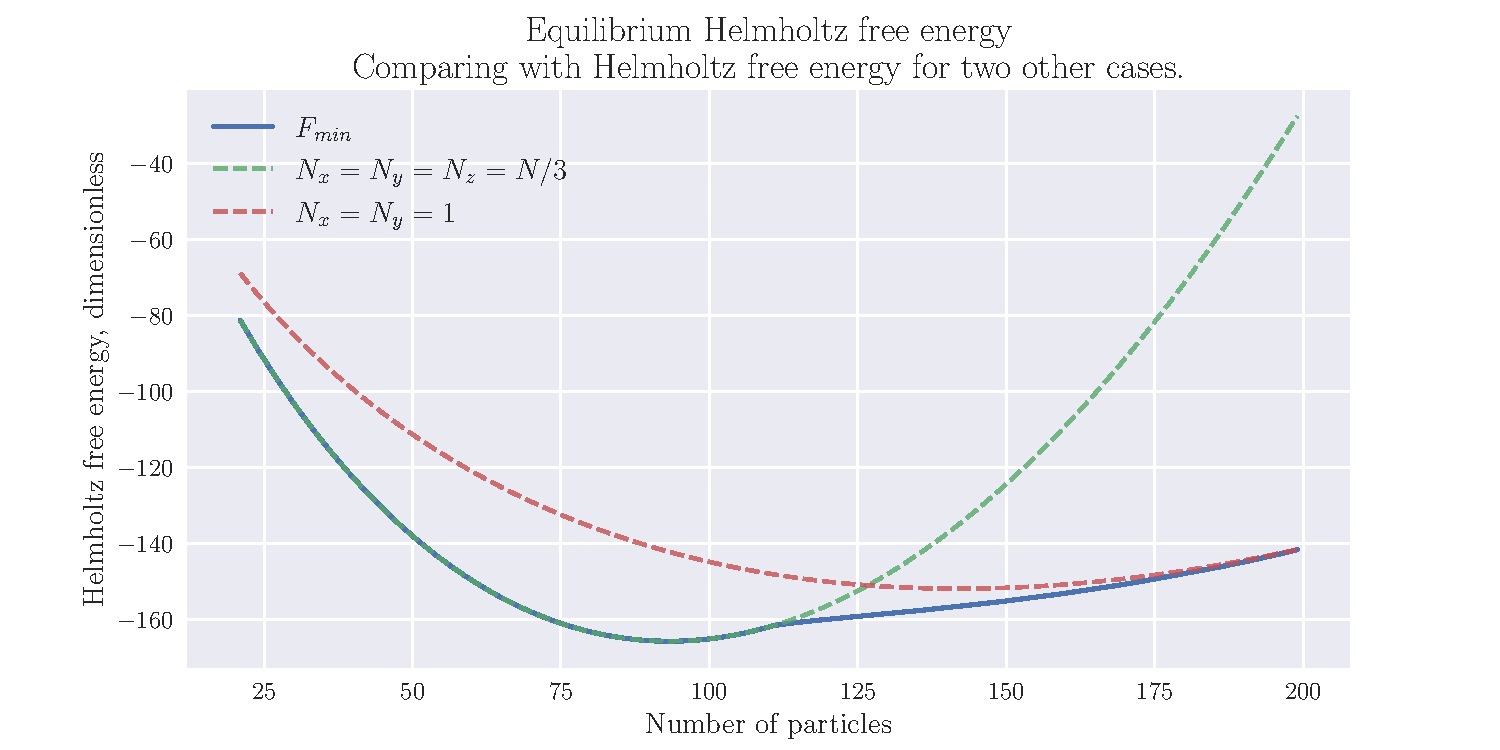
\includegraphics[width=0.8\linewidth]{helmholtz_free_energy.pdf}
	\caption{Helmholtz free energy as a function of $N$ rods.}
	\label{fig:F}
\end{figure}

To get a better view of the change in $F/T$ as $n$ increases, we plot the helmholtz free energy as a function of $\nx$ and $\ny$ for $N=105$ and $N=114$, as shown in the upper an lower panel of figure \ref{fig:F_contour}, respectively. As the rod concentration becomes sufficiently high, the minima of $F/T$ takes place at three different permutations of $\nx,\,\ny$ and $\nz$. 

  

\begin{figure}[h!]
	\centering
	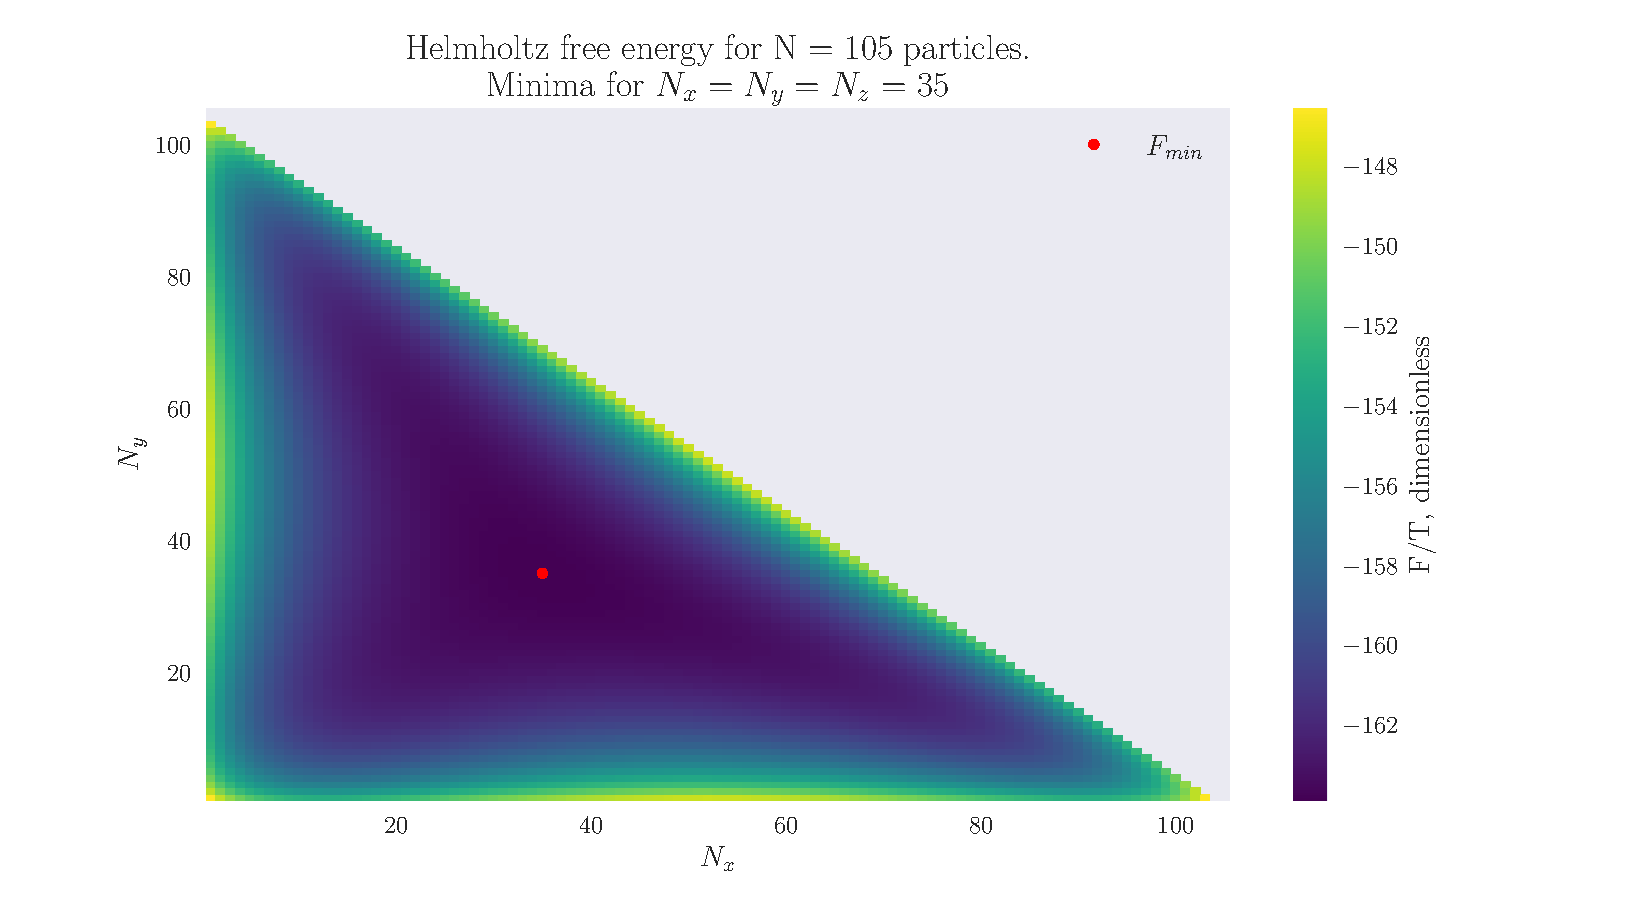
\includegraphics[width=0.9\linewidth]{helmholtz_n105_contour.pdf}
	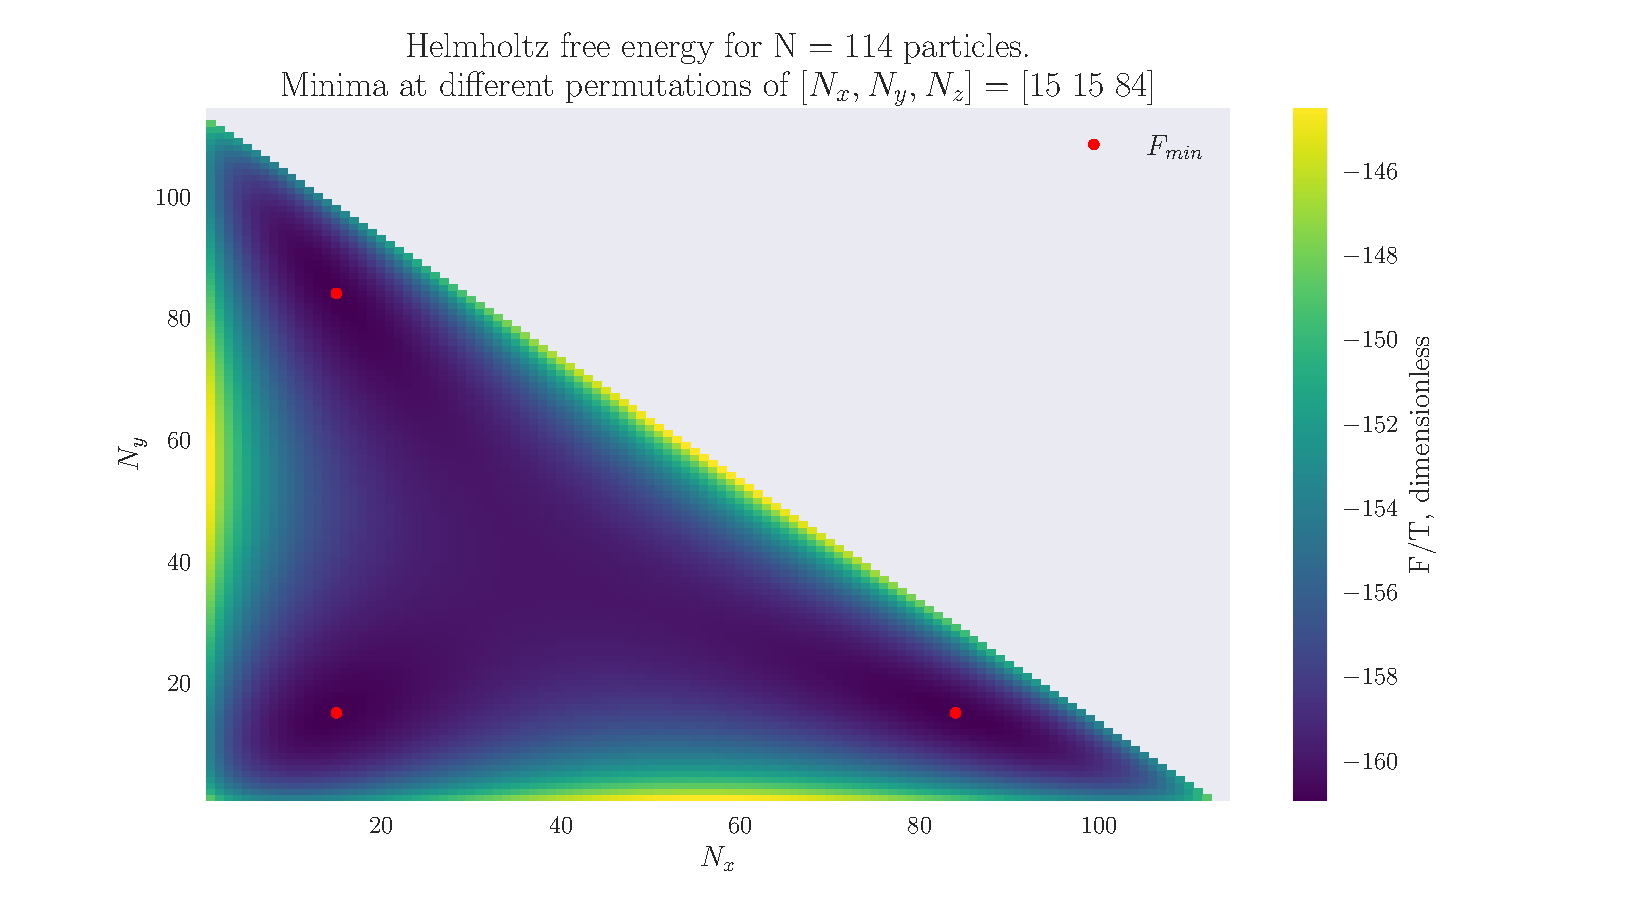
\includegraphics[width=0.9\linewidth]{helmholtz_n114_contour.pdf}
	\caption{The helmholtz free energy at multiple values of $\nx$ and $\ny$ for different number of rods. The upper panel shows the Helmholtz free energy before the phase transition, while the lower panel shows the Helmholtz free energy after.}
	\label{fig:F_contour}
\end{figure}

We can see why this is the case by setting $\nz=N-\nx-\ny$ and differentiate $F/T$ with respect to $\nx$ and $\ny$ and set the two expressions equal to zero to find conditions for minima. Stating the result without deriving it, the condition for minima in terms of $\nx$ and $\ny$ is 
\begin{align*}
	\ln\closed{\frac{\nx}{\ny}}=\gamma \frac{\nx - \nz}{\V}
\end{align*}
This condition is clearly fulfilled when $\nx=\ny$, but for sufficiently large $N$ it will also be fulfilled at $\nx\neq\ny$, which causes this change in $F/T$. Here, we have not discussed $\nz$ and actual values, but the main idea is that $F/T$ will have minimima when the condition $\nx=\ny=\nz$ is not fulfilled. 

We find an expression for the pressure, by taking the partial derivative of $F$ with respect to volume, at constant $T$ and $N$
\begin{align*}
	P &= -\tmdv{F}{V}{T}{N} = -\tmdv{\V}{V}{T}{N}\tmdv{F}{\V}{T}{N}=-\frac{1}{lb^2}\tmdv{F}{\V}{T}{N}
\end{align*}
We now define the dimensionless pressure, $\P\equiv Plb^2/T$, and can then differentiate equation \eqref{eq:F_dimless} with respect to $\V$.
\begin{align}
	\P &= -\bracket{-\frac{\nx}{\V} -\frac{\ny}{\V} -\frac{\nz}{\V} - \gamma \frac{\nx\ny+\ny\nz+\nz\nx}{\V^2}} \nonumber \\ 
	& = \frac{N}{\V} + \gamma \frac{\nx\ny+\ny\nz+\nz\nx}{\V^2} \label{eq:dimless_pressure}
\end{align}
From equation \eqref{eq:dimless_pressure} we see that a significant decrease of two rod orientations with a simultaneous increase in a third yields a lower pressure compared to the case with equal orientation distribution.  

For low values of $N$, there will be numerous minima where the total number of rod is not a multiple of $3$ and we get small oscillations in the relative orientation distribution. A plot of this distribution is shown in figure \ref{fig:F_N}, and shows how there are oscillations apparent at first, but as a critical point is reached, the rods are mostly oriented in the $x$ direction. Here, we clearly see the phase transition going from an equal rod distribution to a $\nx$ completely dominating. This is just one of three possible phase transitions since one of the other orientations are also minima. Coexistence of phases could occur for this model. The value of $\V$ in our model is quite low, but if we were to increase $\V$ enough, such that $n$ almost increases continuously as we increase $N$, there would be a value of $N$ where the Helmholtz free energy is minimized at $\nx=\ny=\nz$ and at the other three possibilities simultaneously. 

In figure \ref{fig:F_N}, the abrupt increase in $\nx$ at $N\sim110$ is a critical point. As we add more rods, there are further discontinuous changes in concentraions where $\nx/N$ increases stepwise until we reach a unidirectional orientation. 

\begin{figure}[h!]
	\centering
	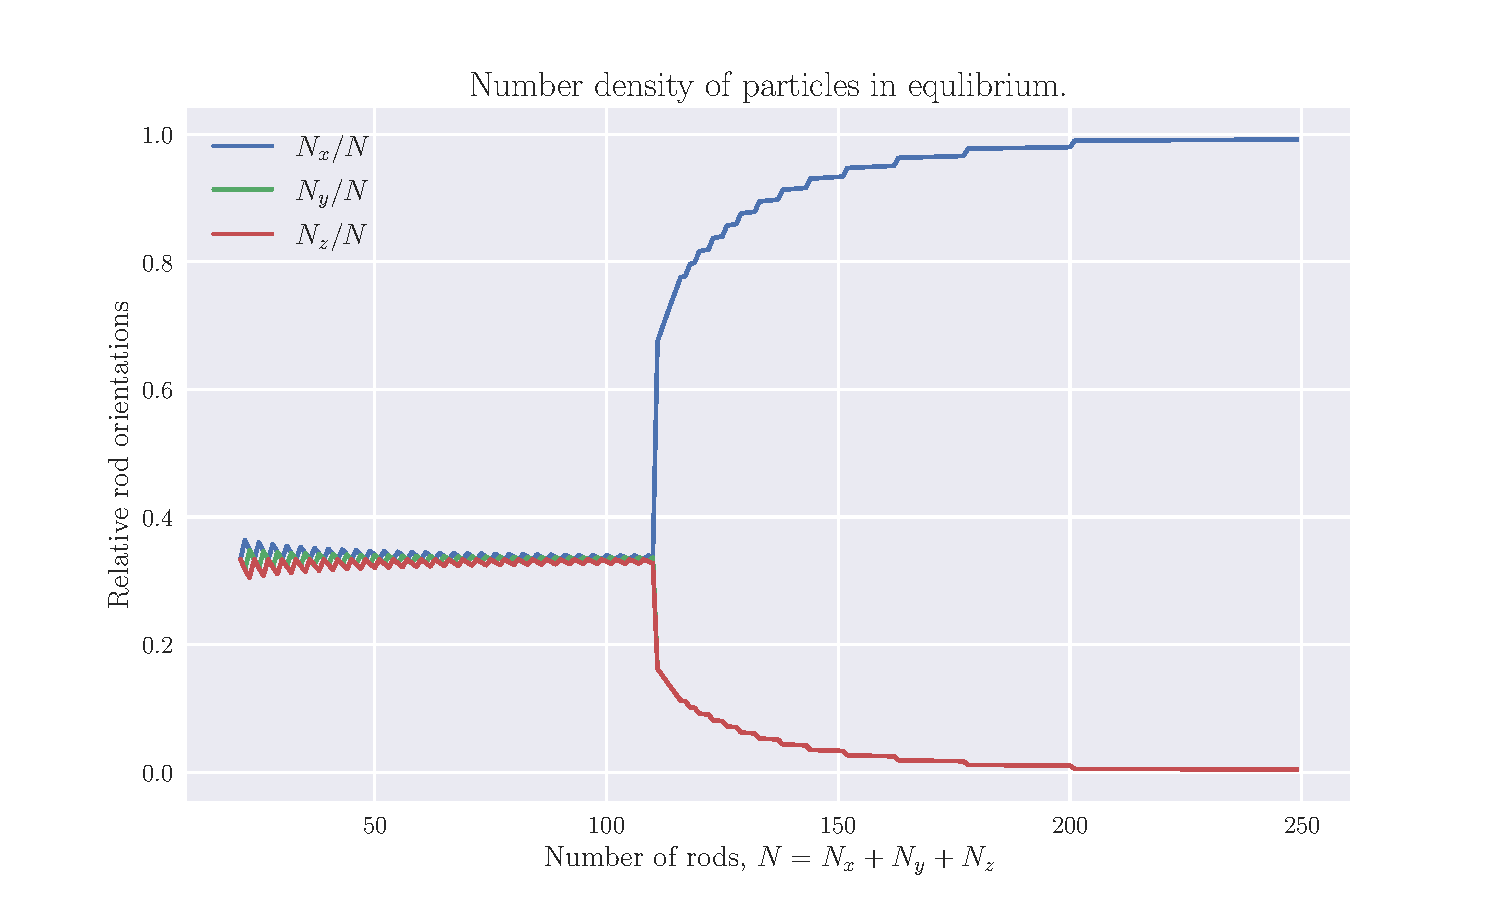
\includegraphics[width=0.8\linewidth]{helmholtz_number_density.pdf}
	\caption{Orientation distribution as we add rods}
	\label{fig:F_N}
\end{figure}

To see how the pressure changes, we plot the pressure from equation \eqref{eq:dimless_pressure} as a function of $N$, shown in figure \ref{fig:F_P}. We see how the pressure increases continuously at first before it drops after the first phase transitions. Increasing $n$ further, the pressure increases until there is an increase in $\nx/N$. 


\begin{figure}[h!]
	\centering
	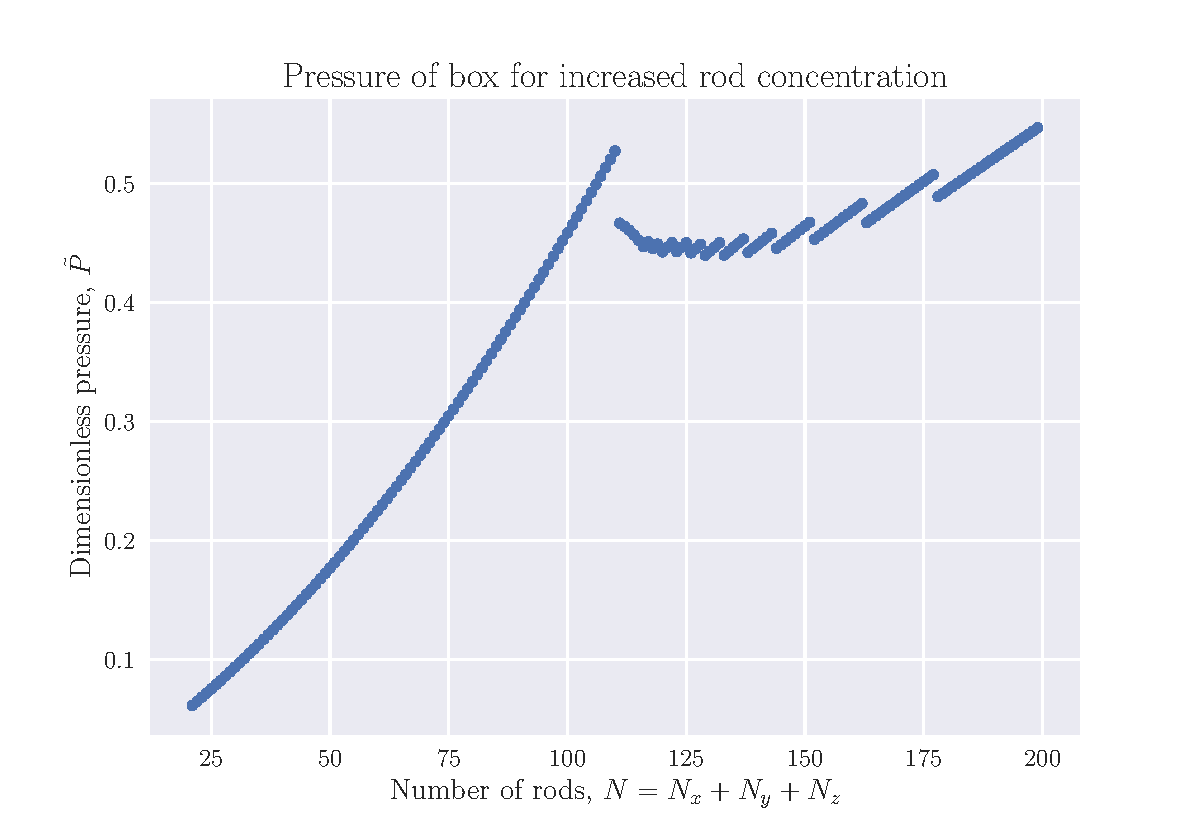
\includegraphics[width=0.8\linewidth]{helmholtz_pressure.pdf}
	\caption{Pressure of the box as we add rods}
	\label{fig:F_P}
\end{figure}

There are four quantities that changes discontinuously as we $n$ is continuously increased. We have not increased $n$ continuously in this, the situation is identical for much larger values of $\V$ and subsequently $N$, where we can view it as being continuous. There appears to be a  discontinuous change in $F/T$ with a sudden change in inclenation as we reach the critical concentration. From figure \ref{fig:F_P} we see clear discontinuous changes in the pressure at each instance where rod orientations change. Since $F\propto T$, we see that the entropy is identical to our dimensionless expression for $T$. Thus, there is a discontinuous change in entropy as well. For the chemical potential we can consider the change in $F/T$ for e.g. $\nx$. Although $F/T$ may appear continuous, at the phase transition there is a discontinuous change in $N_x$ yielding a discontinuous change in the relevant chemical potential as well. At low $n$ there is an equal amount of energy required when adding a rod, independent of its orientation. As the rods align, however, there will be different amounts of energy required to add a rod parallell to the others, compared to a different direction.   

\subsection*{c) - Equilibrium Gibbs free energy}
The Gibbs free energy is given as $G=F+PV$. Using the dimensionless pressure from equation \eqref{eq:dimless_pressure} we can find the dimesnionless Gibbs free energy, $G/T$
\begin{align*}
	\frac{G}{T} &= \frac{F}{T} + \frac{PV}{T} = \frac{F}{T} + \P\V \\
	&= N_x \ln\closed{\frac{N_x}{\tilde{V}}} + N_y \ln\closed{\frac{N_y}{\tilde{V}}} + N_z \ln\closed{\frac{N_z}{\tilde{V}}} + 2\gamma \frac{\nx\ny+\ny\nz+\nz\nx}{\tilde{V}} + N 
\end{align*}
We increase the pressure by decreasing the volume, starting at $V_0=10N$ and ending at $V_\mathrm{max}=2N$ using $N=180$ rods. For each reduction in volume, we find the orientations that minimize $G/T$. We plot the resulting equilibrium Gibbs free energy as a function of $\P$, as shown in figure \ref{fig:G}, where we once again have chosen $\nx$ to be the largest after \textit{(""if"")} a phase transition occurs. As we increase the pressure, we see the phase transitions as the pressure drops abruptly for increased $G/T$. 

\begin{figure}[h!]
	\centering
	\includegraphics[width=0.8\linewidth]{gibbs_free_energy.pdf}
	\caption{Gibbs free energy for increased pressures}
	\label{fig:G}
\end{figure}

We proceed by plotting the pressure as a function of volume. In figure \ref{fig:G_PV} we see how the pressure drops as we reach certain volumes. This corresponds to the orientations of rods changing from uniformly distributed, to one of them dominating. We see the similar situation as we did for the Helmholtz free energy, where there are multiple phase transitions as the rods start to align in the same direction.  
\begin{figure}[h!]
	\centering
	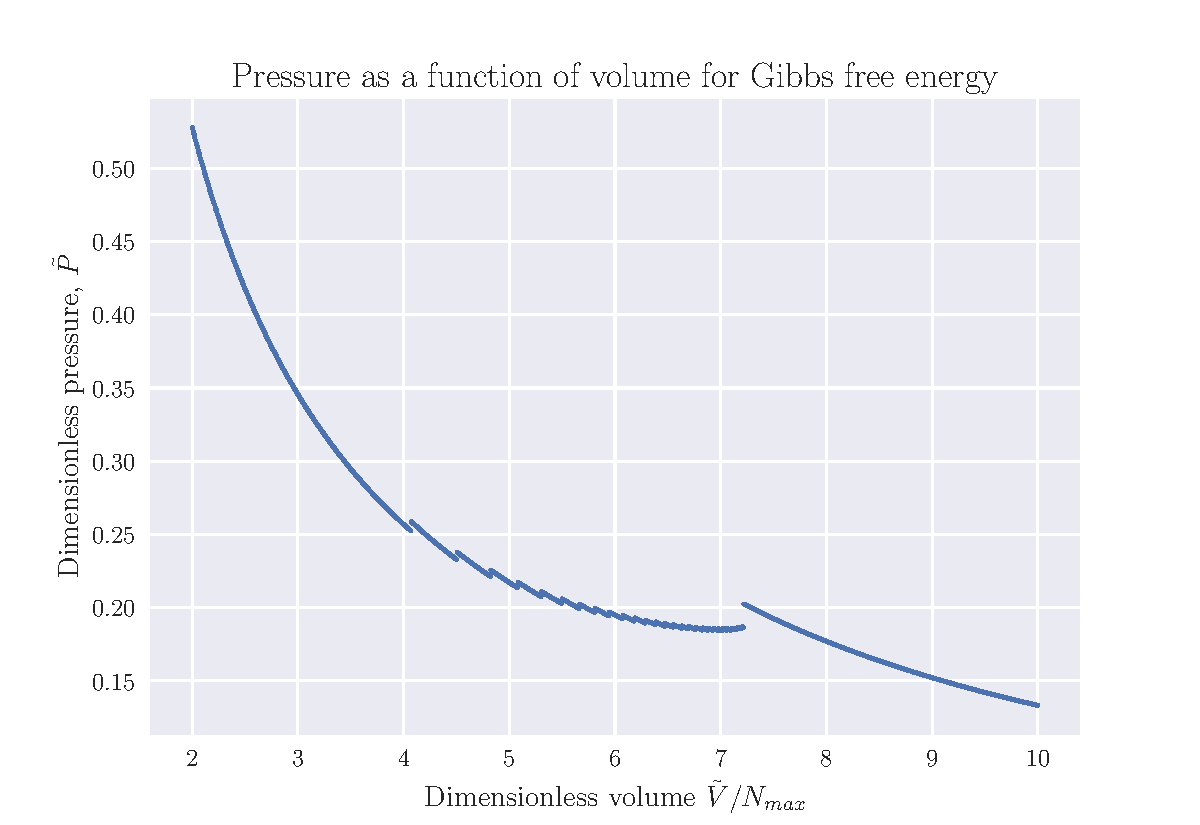
\includegraphics[width=0.8\linewidth]{gibbs_PV.pdf}
	\caption{Pressure as a function of decreasing volume}
	\label{fig:G_PV}
\end{figure}

We plot the relative concentration once more, and see the same situation in figure \ref{fig:G_N} as we did before, where the rods eventually align.  
\begin{figure}[h!]
	\centering
	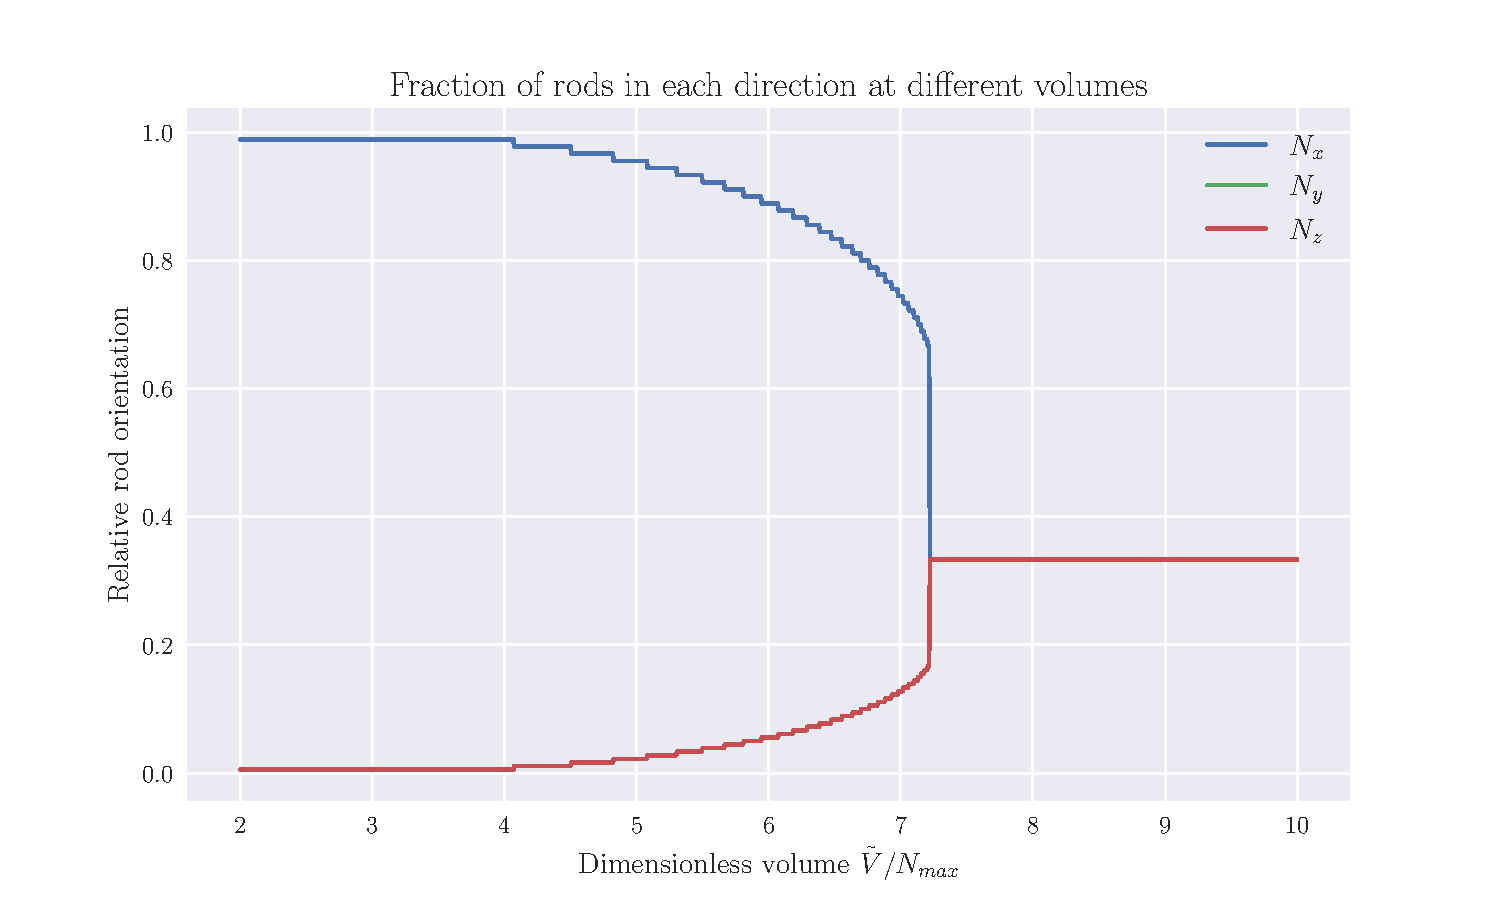
\includegraphics[width=0.8\linewidth]{gibbs_number_density.pdf}
	\caption{Orientation distribution of particles as volume is decreased.}
	\label{fig:G_N}
\end{figure}

The same arguments that were considered before apply for the quantities changing discontinuously as $P$ increases, that is, $G$, $S$ and $\mu$ changes discontinuously. However, the volume is no longer held constant, and is clearly changing discontinuously. 

\clearpage
\section*{\large Task 4}
We consider the system of $N$ independent internal energies with energy values $\pm J$, corresponding to $\np$ and $N_-$, with the constraint $N=\np + N_-$. The total energy of the system is given by
\begin{align} \label{eq:task4_energy}
	E=J(\np-N_-)
\end{align}

\subsection*{a)}
The system we're considering is analogous to a toin coss, and we find the number of different micrstates from the binomial coefficient, where the constrain $\np+N_-=N$ can be used to eliminate $N_-$
\begin{align*}
	\Omega(N,\np) = \frac{N!}{\np!N_-!}=\frac{N!}{\np!(N-\np)!}
\end{align*}


\subsection*{b)}
To find the entropy as a function for $T$ and $N$ where we assume large $N$, we start by taking the logarithm of $\Omega(N,\np)$ and use Stirling's approximation on the different terms. 
\begin{align*}
	\ln\Omega(N,\np) &= \ln(N!) - \ln(\np!)-\ln(N-\np)! \\ 
	&\approx N\ln N - \np \ln\np - (N-\np)\ln(N-\np) - N + \np + (N-\np) \\
	&=N\ln N - \np \ln\np - (N-\np)\ln(N-\np)
\end{align*}
We want to eliminate $\np$ from the expression in favor of temperature. To do this, we will take the partial derivative of $S$ with respect to $E$
\begin{align*}
	\frac{1}{T}=\tmdv{S}{E}{V}{N}=\tmdv{\np}{E}{V}{N}\tmdv{S}{\np}{V}{N}
\end{align*}
Rewriting equation \eqref{eq:task4_energy} in terms of $\np$ and $N$ yields an expression for the derivative of $\np$ with respect to $E$
\begin{align*}
	E = J(2\np-N) \implies& \np = \frac{1}{2}\closed{\frac{E}{J}+N} \\ 
	\tmdv{\np}{E}{V}{N} =&\;\; \frac{1}{2J}
\end{align*}
Using the definition of entropy, $S = \kb \ln\Omega(N,\np)$, we differentiate that with respect to $\np$, where we use the approximated expression for $\ln\Omega(N,\np)$

\begin{align*}
	\tmdv{S}{\np}{V}{N} &= \kb \pdv{\np}\bracket{N\ln N - \np\ln\np - (N-\np)\ln(N-\np)} \\ 
	&= \kb \bracket{-\ln\np - 1 + \ln(N-\np) + 1} \\ 
	&= \kb\ln\closed{\frac{N-\np}{\np}}
\end{align*}
Putting the pieces back together, we get 
\begin{align}
	\frac{1}{T} &= \frac{1}{2J} \kb \ln\closed{\frac{N-\np}{\np}} \\ 
	\ln\closed{\frac{N-\np}{\np}} &=\frac{2J}{\kb T} \\ 
	\implies \np = \frac{N}{1+e^{2J/\kb T}} \label{eq:N_plus}
\end{align}
For simplicity, we now define $x\equiv \frac{2J}{\kb T}$. Before we start inserting our expression for $\np$ to obtain the entropy function we find expressions for $\ln\np$, $N-\np$ and $\ln(N-\np)$ in terms of $N$ and $x$. 
\begin{align*}
	\ln\np&=\ln\closed{\frac{N}{1+e^x}} = \ln N - \ln(1+e^x) \\ 
	N - \np &= N\closed{1 - \frac{1}{1+e^x}}=N\closed{\frac{e^x}{1+e^x}}=\frac{N}{1+e^{-x}} \\
	\ln(N-\np) &= \ln\closed{\frac{N}{1+e^{-x}}} = \ln N - \ln(1+e^{-x})
\end{align*}  

Inserting these values for $\ln\Omega(N,\np)$ yields 
\begin{align*}
	S=\kb \ln\Omega(N,\np) &= \kb \bracket{N\ln N - \frac{N}{1+e^x}\closed{\ln N - \ln(1+e^x)} - \frac{N}{1+e^{-x}} \closed{\ln N - \ln(1+e^{-x})}} \\ 
	&=\kb \bracket{N\ln N \closed{1 - \frac{1}{1+e^x} - \frac{1}{1+e^{-x}}} + N\closed{\frac{\ln(1+e^x)}{1+e^x} + \frac{\ln(1+e^{-x})}{1+e^{-x}}}} \\ 
	&= N\kb \bracket{\frac{\ln(1+e^x)}{1+e^x} + \frac{\ln(1+e^{-x})}{1+e^{-x}}}
\end{align*}
To proceed, we simplify further by considering the logarithm in the last term 
\begin{align*}
	\ln(1+e^{-x}) &= \ln(e^{-x}(1+e^x)) = -x + \ln(1+e^x) \\ 
	\implies \frac{1}{1+e^{-x}}\ln(1+e^{-x}) &= \frac{\ln(1+e^x)}{1+e^{-x}} - \frac{x}{1+e^{-x}}
\end{align*}
Having two common factors of $\ln(1+e^x)$, the entropy expression simplifies even further 

\begin{align*}
	S &= N\kb \bracket{\closed{\frac{1}{1+e^x} + \frac{1}{1+e^{-x}}}\ln(1+e^x) - \frac{x}{1+e^{-x}}} \\ 
	&= N\kb \bracket{\ln(1+e^x) - \frac{x}{1+e^{-x}}}
\end{align*}

Inserting the expression for $x$ yields the final entropy expression as a function of $T$ and $N$
\begin{align}
	S(T,N) &= N\kb \bracket{\ln\closed{1+e^{2J/\kb T}} - \frac{2J/\kb T}{1+e^{-2J/\kb T}}}
\end{align}

\subsection*{c)}
To find the heat capacity, we use the chain rule to ease the computation 
\begin{align*}
	C_V &= T\tmdv{S}{T}{V}{N} = T \tmdv{x}{T}{V}{N}\tmdv{S}{x}{V}{N} = -T\frac{2J}{\kb T^2}\tmdv{S}{x}{V}{N} \\ 
	\tmdv{S}{x}{V}{N} &= N\kb \bracket{\frac{e^x}{1+e^x} - \frac{1}{1+e^{-x}} -x \frac{e^{-x}}{(1+e^{-x})^2} } \\ 
	&= - N\kb x \frac{e^x}{(1+e^x)^2} = -N\kb \frac{2J}{\kb T} \frac{e^{2J/\kb T}}{\closed{1+e^{2J/\kb T}}^2}
\end{align*}
Putting it all together, we finally arrive at 
\begin{align*}
	C_V = \frac{4J^2 N}{\kb} \frac{1}{T^2} \frac{e^{2J/\kb T}}{\closed{1+e^{2J/\kb T}}^2}
\end{align*}
Without any explicit calculation, we rewrite the exponential factor in terms of a hyperbolic function 
\begin{align*}
	\frac{e^x}{(1+e^x)^2} &= \frac{1}{4\cosh^2(\frac{x}{2})} \\
	\implies \frac{e^{2J/\kb T}}{\closed{1+e^{2J/\kb T}}^2} &= \frac{1}{4 \cosh^2\closed{\frac{J}{\kb T}}}
\end{align*}
And our final expression for the heat capacity becomes 
\begin{align}
	C_V = \frac{J^2 N}{\kb} \frac{1}{T^2} \frac{1}{\cosh^2\closed{\frac{J}{\kb T}}}
\end{align}

Next, we consider the limits as $T\to\infty$ and $T\to0$. Using $\text{L}\hat{\;}\,\text{Hopital}$, its easy to find that 
\begin{align*}
	\lim_{T\to\infty} C_V(T) = \lim_{T\to0} C_V(T) = 0
\end{align*}
Since we're more interested in the general behaviour of $C_V$, we plot the function 
\begin{align*}
	c (x) &= \frac{1}{x^2} \frac{1}{\cosh^2\closed{\frac{1}{x^2}}}
\end{align*}
which has an identical dependency to $C_V$. 

\begin{figure}[h!]
	\centering
	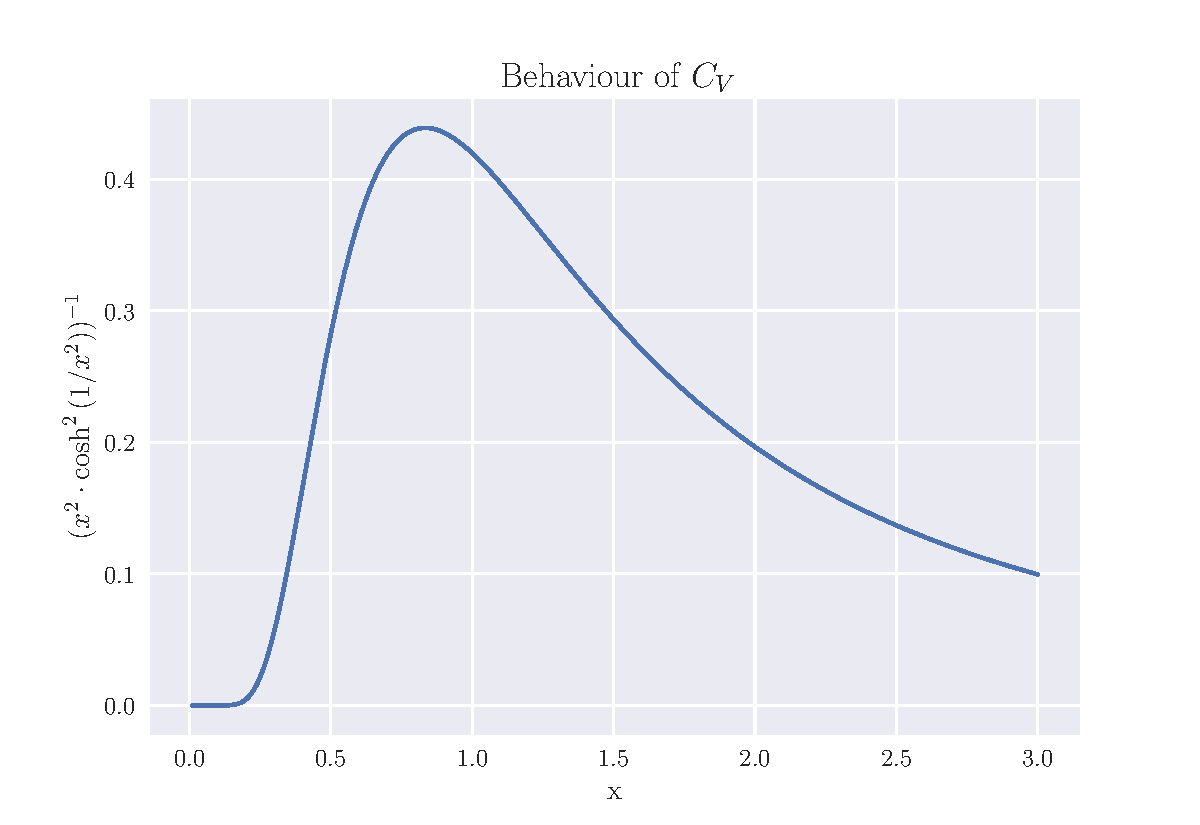
\includegraphics[width=0.49\linewidth]{heat_cap3.pdf}
	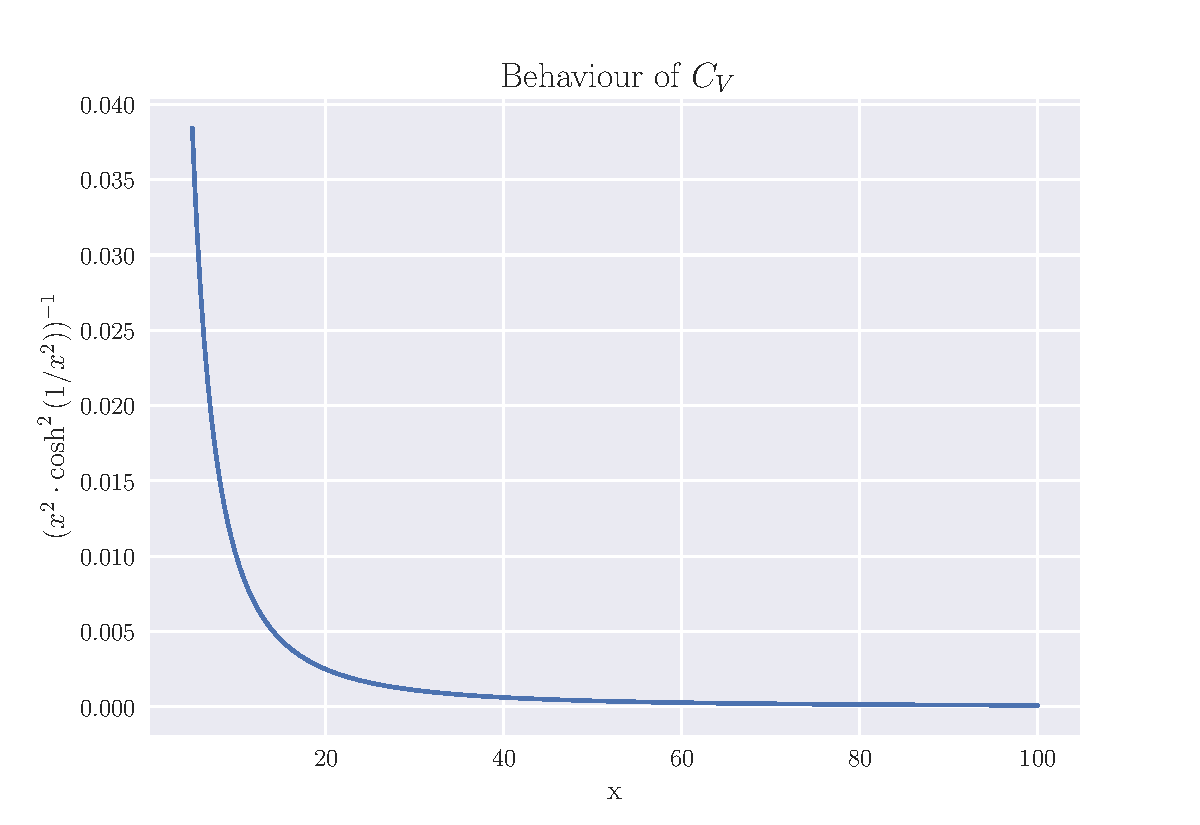
\includegraphics[width=0.49\linewidth]{heat_cap100.pdf}
	\caption{Behaviour of the heat capacity in limiting cases, $c(x)$}
	\label{fig:Cv}
\end{figure}
We see in figure \ref{fig:Cv} that $C_V$ will behave linearly near $T\gtrsim0$. This is also the case for $T>50$, and in both regions we see that it approaches zero. As the temperature increases from $T=0$, there is an increase in heat capacity at first, corresponding to an abrupt increase in entropy. As the temperature surpasses a certain point, increasing $T$ further dampens the increase in $S$ slightly, as as we reach high enough termperature values, the change in entropy is more or less completely absent. By considering the expression for $\np$ in equation \eqref{eq:N_plus} we see that as $T\to 0$ we have $\np\to0$ and for $T\to\infty$ we get $\np\to N$. Thus, as $T\to0$, all the internal degrees of freedom have energy $-J$ resulting in $E=-NJ$. Surpassing the points when $\np=N_-$ such that $E=0$, we eventually arrive at an energy of $E=+NJ$, where all the internal degrees of freedom have energy $+J$. In both limiting cases, the change in entropy is miniscule when we adjust $T$ since all internal degrees of freedom have taken the same energy value.  

\end{document}
